\documentclass[12pt]{article}
\usepackage{graphicx} % for including figure 
\usepackage{geometry} % geometry package for mentioning margin length
\usepackage{hyperref}
\usepackage{amssymb}
\usepackage{amsmath}
\usepackage{wrapfig}
\hypersetup{
    colorlinks=true,
    linkcolor=blue,
    filecolor=magenta,	    
    urlcolor=cyan,
		citecolor=black,
}
\urlstyle{same}
\geometry{margin=3cm} %for setting margin; DON'T CHANGE THIS

\usepackage{bbm}
\usepackage{mathtools}
\usepackage{algorithm}
\usepackage{circuitikz}
\usepackage[noend]{algpseudocode}
% the boxed option keeps the algorithm in a box in the pdf.
% You can also use the option ruled or algoruled for a different output.
% For more information about the algorithm2e package you can read the docuemntation 
% at https://mirror.easyname.at/ctan/macros/latex/contrib/algorithm2e/doc/algorithm2e.pdf

\newcommand{\BigO}{\ensuremath{\mathcal{O}}}
\title{Solving the Maze Problem with Inductive Logic Programming: A comparison between HYPER, Metagol and ILASP}
\author{Angelo Andreussi, Alex Della Schiava, Claudia Mau\ss ner}


\begin{document}
\maketitle

\section{Outline}
In this document, we intend to describe our Inductive Logic Programming (ILP) solutions to the Maze problem.\\
Section~\ref{sec:intro} offers a brief illustration of the Maze Problem we have been working on,
including the main choices and assumptions we made.\\
Section~\ref{sec:back} lists the tools we have used to reach our goal.
\section{Introduction}\label{sec:intro}
Our work is focussed on the Maze problem. This problem consists in finding a path from point \texttt{A}
to point \texttt{B} in a labirinth-like shaped map (see Figure~\ref{fig:fig1}). A variety of classical algorithms
can be used to solve this problem, starting from the most naïve wall following algorithm to more complex and elaborated
ones exploiting graph theory concepts.\\
By approaching this simple problem with ILP though, it is possible to extend it into a much more sophisticated and interesting
problem. For instance, it allowed us to start with the assumption that the problem's main character (the
one we shall refer to as \emph{agent}) has no knowledge about \emph{how} to move. Consequently, before even trying
to solve the Maze, the agent needs to learn what a \emph{move} is and then what a \emph{legal} move is.


\begin{figure}[b]
  \centering
  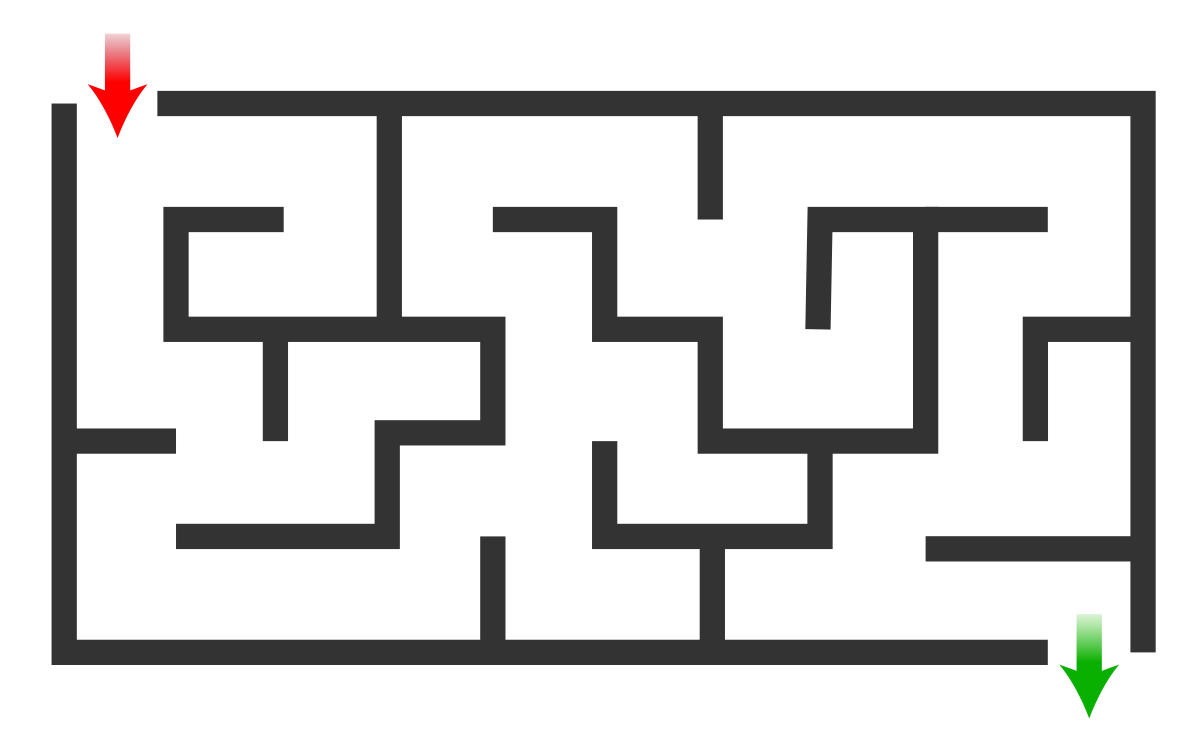
\includegraphics[scale=0.1]{img/Maze_simple.svg.png}
  \caption{Example of a Maze}\label{fig:fig1}
\end{figure}


\section{Background}\label{sec:back}
\section{Implementation}\label{sec:impl}
\subsection{HYPER}
\subsection{Metagol}
\subsection{ILASP}
\section{Performance comparison}


\end{document}
